\section{Tree Extraction}

\begin{figure}[t]
	\centering
	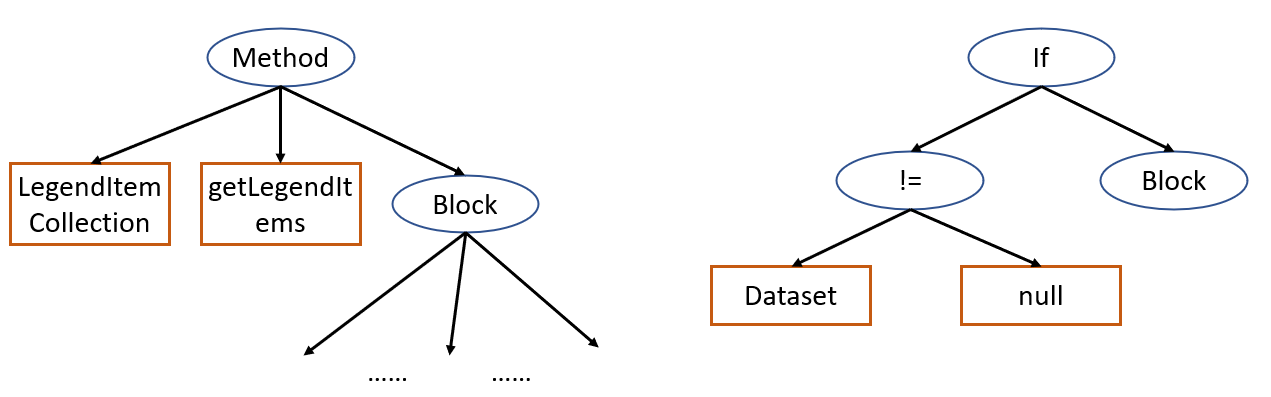
\includegraphics[width=3.2in]{graphs/tree_extraction.png}
	\caption{Abstract Syntax Tree Extraction}
	\label{tree-extraction}
\end{figure}


The first step of the \tool is the tree extraction step designed to extract abstract syntax tree (AST) from the source code. It accepts the buggy method with the changed statements inside as input. The output of this step is the extracted AST for the whole buggy method and the extracted sub-tree of AST that represents the changed statements.

Specifically, for a buggy method $m$, \tool uses the Java package JDT \cite{JDT} to generate the AST to represent the buggy method. And for a buggy statement $s$ in the buggy method, \tool uses the sub-tree of AST that exactly covers the statement $s$ to represent the buggy statement. For example, in Figure \ref{tree-extraction}, the AST in the left represents the buggy method in Figure \ref{fig:motiv}, and the right sub-tree of AST in Figure \ref{tree-extraction} represents the buggy statement. If there is more than one buggy statement in the buggy method $m$, \tool generates multiple sub-tree of AST to represent each buggy statement.

Also, when training the model, \tool needs ground truth to let the model learn the parameters, \tool also generates the AST to represent the fixed method $m_f$ and the sub-tree of AST to represent the fixed statement $s_f$. Here, $m_f$ is the after fixing version of buggy method $m$, and $s_f$ is the after fixing version of buggy statement $s$. Thus, \tool uses the AST and sub-tree of AST for fixed method and fixed statement as the ground truth to train the model parameters.

For the buggy method, $m$ and corresponding fixed method $m_f$, \tool can easily find them from the dataset based on the true labels. However, pairing the buggy statement $s$ with its corresponding fixed version $s_f$ is not easy as the methods. To solve this problem, we use an existing approach CPatMiner \cite{nguyen2019graph} to process the fixing changes. Based on the results from CPatMiner, we pair the buggy statement $s$ with the corresponding fixed statement $s_f$ within the three following conditions. 1) If the buggy statement $s$ needs to be deleted, we pair $s$ with an empty statement. 2) if the buggy statement $s$ needs to be updated, we pair $s$ with the updated statement. 3) If there needs to insert a new statement as the fixing, we check the AST for the method $m$ first. And we pair the parent node with the inserted statement $s_f$ if the parent node representing the other statement, or we pair an empty statement with the inserted statement $s_f$. 